% SOM architecture figure for the TorchSOM documentation.
% Input features x_1..x_k fully connected to an m x n grid of neurons w_ij.
% Recovered from the JMLR paper history (commit b970394) and kept here so the
% docs figure stays reproducible.
%
% Regenerate the PNG with:
%   pdflatex architecture.tex
%   pdftocairo -png -singlefile -r 300 architecture.pdf ../source/_static/som/architecture
\documentclass[tikz,border=4pt]{standalone}
\usepackage{amssymb}

% Layout parameters (mirror the paper's imports.tex).
\def\xspace{2}    % horizontal spacing
\def\yspace{1.5}  % vertical spacing
\def\xoffset{3}   % horizontal offset to centre the SOM grid
\def\yoffset{0}   % vertical offset
\def\m{3}         % rows
\def\n{3}         % columns

\begin{document}
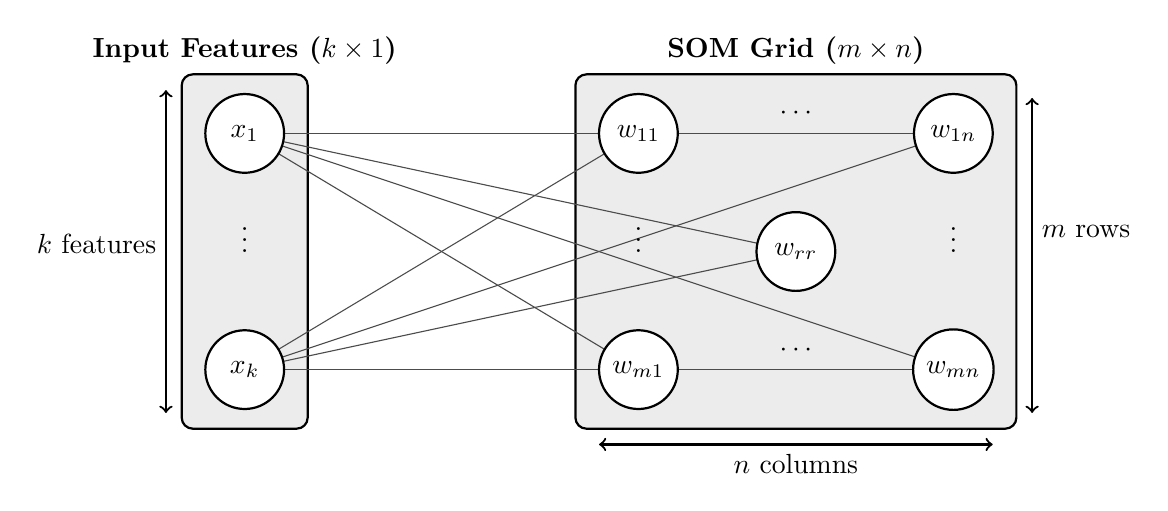
\begin{tikzpicture}[scale=1, every node/.style={scale=1}]
    % Input features: only the 1st and kth (last) are drawn.
    \coordinate (x1) at (0, {-(1-0.5)*\yspace-1});
    \coordinate (xk) at (0, {-(3-0.5)*\yspace-1});
    % SOM grid weights, sharing the y-coordinates of x1 and xk.
    \foreach \j in {1,...,\n} {
            \foreach \i in {1,...,\m} {
                    \coordinate (w\i\j) at ({\j*\xspace + \xoffset}, {-(\i-0.5)*\yspace-1});
                }
        }

    % "Input Features" box.
    \draw[thick, rounded corners, fill=gray!15] (-0.8, {1+-1*\yspace-0.5}) rectangle (0.8, {-0.5-3*\yspace-0.5});
    \node[above, font=\bfseries] at (0, {1+-1*\yspace-0.5}) {Input Features ($k \times 1$)};
    % "SOM Grid" box.
    \draw[thick, rounded corners, fill=gray!15]
    ({1*\xspace + \xoffset - 0.8}, {1+-1*\yspace-0.5}) rectangle
    ({3*\xspace + \xoffset + 0.8}, {{-0.5-3*\yspace-0.5}});
    \node[above, font=\bfseries] at ({2*\xspace + \xoffset}, {1+-1*\yspace-0.5}) {SOM Grid ($m \times n$)};

    % Connections from the first and last feature to corner and centre neurons.
    \draw[black!70, ->] (x1) -- (w11);
    \draw[black!70, ->] (x1) -- (w\m\n);
    \draw[black!70, ->] (x1) -- (w1\n);
    \draw[black!70, ->] (x1) -- (w\m1);
    \draw[black!70, ->] (x1) -- (w22);
    \draw[black!70, ->] (xk) -- (w11);
    \draw[black!70, ->] (xk) -- (w\m\n);
    \draw[black!70, ->] (xk) -- (w1\n);
    \draw[black!70, ->] (xk) -- (w\m1);
    \draw[black!70, ->] (xk) -- (w22);

    % Input feature nodes.
    \node[circle, draw, thick, minimum size=10mm, fill=white] (node1) at (x1) {$x_{1}$};
    \node at (0, -3) {$\vdots$};
    \node[circle, draw, thick, minimum size=10mm, fill=white] (nodek) at (xk) {$x_{k}$};
    % SOM grid neurons: corners and centre.
    \node[circle, draw, thick, minimum size=10mm, fill=white] at (w11) {$w_{11}$};
    \node[circle, draw, thick, minimum size=10mm, fill=white] at (w1\n) {$w_{1n}$};
    \node[circle, draw, thick, minimum size=10mm, fill=white] at (w\m1) {$w_{m1}$};
    \node[circle, draw, thick, minimum size=10mm, fill=white] at (w\m\n) {$w_{mn}$};
    \node[circle, draw, thick, minimum size=10mm, fill=white] at (w22) {$w_{rr}$};

    % Vertical dots for the left and right columns.
    \node at ({1*\xspace + \xoffset}, {-2*\yspace+\yoffset}) {$\vdots$};
    \node at ({3*\xspace + \xoffset}, {-2*\yspace+\yoffset}) {$\vdots$};
    % Horizontal dots for the top and bottom rows.
    \node at ({2*\xspace + \xoffset}, {-1*\yspace+\yoffset}) {$\cdots$};
    \node at ({2*\xspace + \xoffset}, {-3*\yspace+\yoffset}) {$\cdots$};

    % Column count arrow.
    \draw[<->, thick] ({1*\xspace + \xoffset - 0.5}, {-3*\yspace - 1.2+\yoffset}) -- ({3*\xspace + \xoffset + 0.5}, {-3*\yspace - 1.2+\yoffset});
    \node[below] at ({2*\xspace + \xoffset}, {-3*\yspace - 1.2+\yoffset}) {$n$ columns};
    % Row count arrow.
    \draw[<->, thick] ({3*\xspace + \xoffset + 1.0}, {-1.2*\yspace + 0.5+\yoffset}) -- ({3*\xspace + \xoffset + 1.0}, {-3*\yspace - 0.8+\yoffset});
    \node[right] at ({3*\xspace + \xoffset + 1.0}, {-2*\yspace+\yoffset}) {$m$ rows};
    % Feature count arrow.
    \draw[<->, thick] (-1, {0.8-1*\yspace-0.5}) -- (-1, {-0.3-3*\yspace-0.5});
    \node[left] at (-1., {-2.1*\yspace}) {$k$ features};
\end{tikzpicture}
\end{document}
